\chapter{Implementacja części programowej}

\section{Rozszerzenia czasu rzeczywistego}

\par Spośród dostępnych rozszerzeń czasu rzeczywistego można wyróżnić trzy,
najbardziej popularne i sprawdzone opcje:
\begin{enumerate}

    \item Zestaw łatek PREEMPT\_RT - zestaw modyfikacji jądra Linux mających
    na celu rozszerzenie standardowych funkcjonalności o możliwość
    realizacji zadań w czasie rzeczywistym.

    \item Xenomai - środowisko programistyczne pracujące wspólnie 
    z jądrem Linux, umożliwiające tworzenie zadań pracujących w czasie 
    rzeczywistym z deterministycznym czasem realizacji równolegle 
    z zadaniami jądra. Działanie opiera się na stworzeniu mikrojądra obok
    głównego, obsługującego jedynie krytyczne zadania.

    \item RTAI (ang. \textit{Real-Time Application Interface}) - podobnie jak Xenomai,
    zapewnia zestaw interfejsów pozwalających na realizację krytycznych zadań z użyciem
    drugiego jądra, które w przeciwieństwie do środowiska Xenomai, nie jest realizowane 
    w architekturze mikrojądra.

\end{enumerate}

Dokonując analizy dostępnych opcji zdecydowano się na wykorzystanie zestawu 
łatek PREEMPT\_RT. Xenomai i RTAI, mimo że bardzo cenione i często wykorzystywane
w nawet rozwiązaniach komercyjnych, cechują się wysokim progiem wejścia 
i praca z nimi wymaga dużego nakładu czasowego. 

\subsubsection{Zestaw łatek PREEMPT\_RT}

Jądro systemu Linux jest wielozadaniowe i implementuje planistę (ang. \textit{scheduler}), 
którego zadaniem jest szeregowanie i obsłużenie zadań na podstawie ich priorytetu.
Planista decyduje o przydziale czasu procesora na wykonanie zadań, które może przełączać 
w zależności od aktualnego zdażenia lub ustalonego planu.
Standardowo, jądro systemu Linux zapewnia mechanizm wywłaszczenia (ang. \textit{preemption}),
zadania z przestrzeni użytkownia przez zadania o wyższym priorytecie lub przerwania sprzętowe.
Przebieg wywłaszczenia przedstawiono na rysunku \ref{sw::preempt_0}:

\begin{figure}[H]
    \centering
    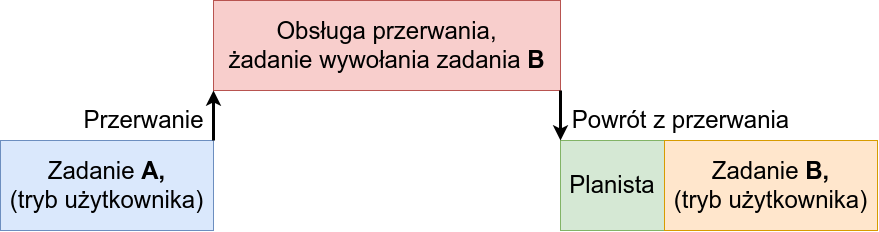
\includegraphics[width=0.75\textwidth]{graf/sw/preempt_0.png}
    \caption{Przebieg wywłaszczenia zadania}
    \label{sw::preempt_0}
\end{figure}

Jako, że jedynie wywłaszczone mogą zostać zadania pracujące w trybie użytkownika, 
nie trudno wyobrazić sobie sytuację, którą przedstawiono na rysunku \ref{sw::preempt_1}

\begin{figure}[H]
    \centering
    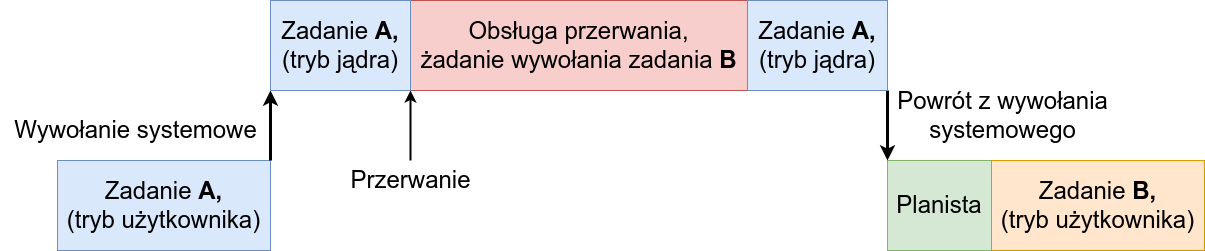
\includegraphics[width=\textwidth]{graf/sw/preempt_1.png}
    \caption{Przebieg wywłaszczenia zadania w sytuacji wywołania systemowego}
    \label{sw::preempt_1}
\end{figure}

Jeżeli przerwanie żądające wywołanie innego zadania nadejdzie w momencie 
wykonywania wywołania systemowego, to takie przerwanie nie zostanie obsłużone 
do momentu jego zakończenia. Oznacza to, że w niektórych sytuacjach 
nie sposób określić czasu potrzebnego na wykonanie pewnego zadania.
Dodatkowo, każde zadanie z przestrzenii użytkownika może zostać wywłaszczone 
przez przerwanie sprzętowe, w którego trakcie niemożliwa jest obsługa innych
przerwań. Oznacza to, że małe ważne przerwania sprzętowe mogą wywłaszczyć
krytyczne czasowo zadania czasu rzeczywistego.
\par Z realizacją wywłaszczeń realizowanych w standardowym systemie Linux wiąże się 
również problem nazywany inwersją priorytetów (ang. \textit{priority inversion}).
Opiera się on na sytuacji, kiedy niekrytyczne zadanie blokuje dostęp (ang. \textit{mutex}) do 
zasobów zadaniu krytycznemu. Przebieg takiego problemu przedstawiono na rysunku \ref{sw::prior_inv}:

\begin{figure}[H]
    \centering
    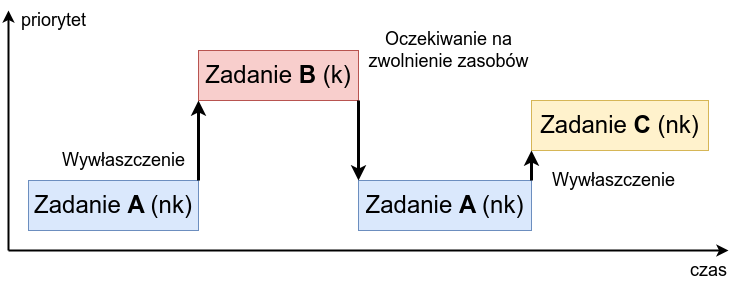
\includegraphics[width=0.8\textwidth]{graf/sw/prior_inv.png}
    \caption{Przebieg problemu inwersji priorytetów}
    \label{sw::prior_inv}
\end{figure}

Krytyczne zadanie \textbf{B} musi uzyskać dostęp do zasobów blokowanych przez zadanie \textbf{A}
o niższym priorytecie. W celu ich odblokowania, 
planista przełącza kontekst na zadanie \textbf{A} lecz w czasie jego wywoływania
zostaje ono wywłaszczone przez zadanie \textbf{B} o wyższym priorytecie.

\section{System operacyjny}

Proces uruchomienia systemu operacyjnego GNU/Linux na wybranej
platformie obliczeniowej przedstawiono na rysunku \ref{sw::boot_process}:

\begin{figure}[H]
    \centering
    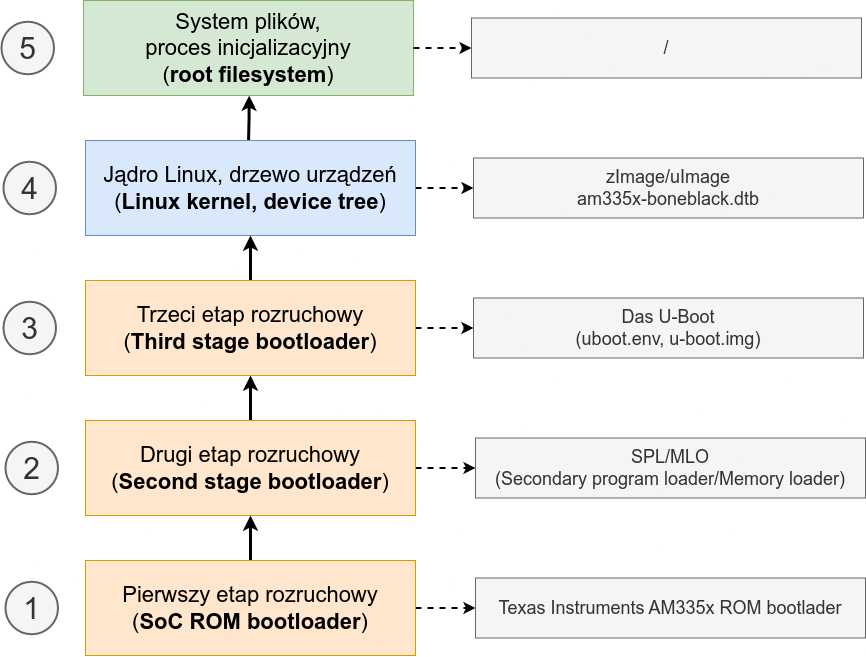
\includegraphics[width=0.8\textwidth]{graf/sw/boot_process.png}
    \caption{Proces uruchomienia systemu operacyjnego}
    \label{sw::boot_process}
\end{figure}

Opis poszczególnych etapów przedstawiono poniżej:
\begin{enumerate}

    \item Pierwszy etap rozruchowy (ang. \textit{Boot ROM}) - jego zadanie polega na 
    inicjalizacji podstawowych magistral i peryferiów niezbędnych do dalszych etapów rozruchu.
    Znajduje się z zafiksowanej przestrzenii adresowej z uprawnieniami
    tylko do odczytu, z której procesor bezpośrednio po uruchomieniu zaczyna
    wykonywać instrukcje.    
    Po inicjalizacji, jego zadaniem jest załadowanie następnego w koleji 
    programu rozruchowego (plik SPL lub MLO) z pamięci zewnętrznej (eMMC, karta microSD) lub
    przez określony protokół cyfrowy (SPI, UART) do wewnętrznej pamięci SRAM procesora.
    Jako, że program znajduje się w pamięci tylko do odczytu, nie podlega 
    modyfikacji.

    \item Drugi etap rozruchowy - kontynuuje inicjalizację peryferiów 
    procesora oraz ładuje trzeci program rozruchowy (plik u-boot.img), wymagający najwięcej
    miejsca do pamięci DDR. Po załadowaniu, przekazuje mu pełną kontrolę. 

    \item Trzeci etap rozruchowy - ładuje jądro wraz z drzewem urządzeń do pamięci DDR oraz 
    inicjalizuje peryferia, które mogą zostać do tego wykorzystane 
    (I2C, NAND, FLASH, Ethernet). Proces ładowania należy odpowiednio skonfigurować,
    wskazując programowi miejsce, w który znajduje się obraz jądra oraz adres
    w pamięci, do którego ma je załadować. Konfiguracji można dokonywać statycznie,
    poprzez uprzednio przygotowany plik (uEnv.txt, uboot.env) lub dynamicznie, 
    wpisując polecenia na etapie działania programu.

    \item Jądro - wykonuje, planuje i zarządza procesami. Jest pośrednikiem
    między interakcjami ze sprzętem (peryferiami), kontrolując je za pośrednictwem
    sterowników, które mogą być osadzone statycznie lub ładowane dynamicznie w postaci modułów.
    Po uruchomieniu i przeprowadzeniu procesu inicjalizacji, włącza
    programy startowe i umożliwia użytkownikowi pracę. Zadania wykonywane przez jądro
    zawierają się w tak zwanej przestrzenii jądra 
    (ang. \textit{kernel space}), która tworzy osobną przestrzeń adresową niedostępną
    dla aplikacji użytkownika. 

    \item Główny system plików - zawiera zestaw plików i katalogów, niezbędnych do działania 
    systemu. Z tego miejsca wychodzą pozostałe struktury katalogów, które definiują 
    obszar roboczy użytkowników systemu wraz z aplikacjami, z których korzystają.

\end{enumerate}

\subsection{Środkowisko pracy}

Tworząc oprogramowanie na platformę wbudowaną należy pamiętać, że architektura 
procesorów na takich urządzeniach różni się od tych typowo wykorzystywanych 
w komputerach personalnych. Chcać skompilować działający program pod daną architekturę, 
niezbędny będzie odpowiedni zestaw narzędzi (ang. \textit{toolchain}), w któreg skład wchodzi
zestaw kompilatorów, konsolidatorów i bibliotek standardowych wykorzystywanego języka.
Wykorzystana w projekcie platforma zaopatrzona jest w procesor ARM Cortex-A8,
więc niezbędny jest zestaw narzędzi zdolnych budować programy pod taką architekturę.
Taki proces przyjeło się nazywać kompilacją skrośną (ang. \textit{cross-compilation}).
\par W projekcie wykorzystano gotowy zestaw narzędzi udostępnianych przez firmę ARM.
W ich skład wchodzi odpowiednio przebudowany GCC oraz zestaw bibliotek standardowych 
języka C i C++. Wszystkie wyszczególnione na rysunku \ref{sw::boot_process} konfigurowalne
etapy ładowania systemu operacyjnego wraz z aplikacją działającą w trybie użytkownia są 
budowane z jego użyciem.

\subsection{Przygotowanie nośnika}

Docelowo, platforma BeagleBone Black ładuje zapisany na etapie 
produkcji system operacyjny z wewnętrznej pamięci eMMC. Chąc wgrać inny system,
wymagane jest zapisanie niezbędnych plików na kartę SD i odpowiednie skonfigurowanie 
płytki, aby przeprowadzała z niej proces ładowania. Aby to wykonać, karta 
SD z plikami systemu operacyjnego musi być odpowiednio podzielona na partycje.
Opis poszczególnych partycji przedstawiono poniżej:

\begin{enumerate}

    \item Partycja rozruchowa - zawiera pliki drugiego i trzeciego programu
    rozruchowego. Wymagany jest system plików FAT32.

    \item Partycja systemowa - zawiera pliki jądra systemu i drzewa urządzeń. Wymagany jest system
    plików EXT4.

    \item Partycja z głównym systemem plików - jak sama nazwa wskazuje, zawiera wypakowany
    główny system plików systemu. Wymagany jest system plików EXT4.

\end{enumerate}

\subsection{Programy rozruchowe}

Pierwszy program rozruchowy jest wgrany przez producenta na etapie produkowania 
układu, więc jest to część systemu, na którą programista nie ma wpływu. Pozostałe 
dwa programy, czyli odpowiednio drugi i trzeci etap rozruchowy, muszą być
odpowiednio skonfigurowane i umiejscowione na odpowiedniej partycji docelowego nośnika,
aby proces uruchomienia systemu odbył się prawidłowo. Jako program rozruchowy zapewniający 
drugi i trzeci etap wybrano pakiet \textit{Das U-Boot}, który stanowi podstawowe 
rozwiązanie dla wbudowanych systemów operacyjnych.
\par Proces budowania poszczególnych etapów przedstawionych na rysunku \ref{sw::boot_process} 
zazwyczaj wygląda bardzo podobnie i można go podzielić na trzy główne kroki:

\begin{enumerate}

    \item Pobranie kodów źródłowych z repozytorium twórców - jeżeli oprogramowanie
    udostępniane jest na licencjach otwartoźródłowych, to twórcy zwyczajowo
    magazynują wszystkie kody źródłowe programu na ogólnodostępnych w internecie repozytoriach.

    \item Konfiguracja procesu budowania - może się różnić w zależności od 
    wykorzystywanego przez program systemu budowania. Typowo, procesowi należy
    wskazać plik konfiguracyjny z charakterystyką używanej platformy.

    \item Budowanie - proces kompilacji zakończony generacją odpowiedniego pliku 
    wykonywalnego.

\end{enumerate}

Platforma BeagleBone Black, jako że jest popularnym układem, posiada już odpowiednio
przygotowane pliki konfiguracyjne dla drugiego etapu budowania, więc dodatkowa 
ingerencja w proces konfiguracji nie jest wymagana. Wynikiem pomyślnego zbudowania 
programu są pliki MLO i u-boot.img, będące odpowiednio drugim i trzecim programem rozruchowym. 
Po wgraniu plików na partycję rozruchową nośnika i uruchomieniu ładowania, 
trzeci program rozruchowy przedstawi się linią poleceń i wymagane będzie wpisanie 
kilku komend, informujących program, skąd i gdzie ma załadować pliki jądra systemu.
Po zapisaniu konfiguracji, programy rozruchowe nie wymagają dodatkowych modyfikacji.

\subsection{Jądro Linux}

Proces budowania jądra Linux jest analogiczny jak proces budowania programów 
rozruchowych. Dodatkową opcją jest możliwość interaktywnej konfiguracji 
budowanego systemu w oparciu o narzędzie \textit{menuconfig}, jednak
domyślny plik konfiguracyjny, opisujący wybraną platformę na potrzeby realizowanego
projektu jest wystarczający.
\par Jedyną zmianą, którą wprowadzono w kodach źródłowych jądra było 
dodanie prostego sterownika obsługującego zaprojektowaną płytkę drukowaną na bazie
kodeku PCM5102A \cite{bib:sitara}. Z najbardziej znaczących kwestii, 
sterownik zawiera deklarację struktury opisującą
konfigurację płytki dla transferów wejściowych i wyjściowych oraz funkcję, 
która umożliwia jego załadowanie i widoczność w systemie.
W wykorzystanym rozwiązaniu napisany moduł bezpośrednio zastąpił sterownik kodeka PCM5102A,
zachowując początkową nazwę, więc dodatkowe modyfikacje w plikach konfiguracyjnych 
jądra nie były konieczne.

\par Proces zastosowania zestawu łatek PREEMPT\_RT można wykonać manualnie, lub 
skorzystać z gotowej opcji przygotowanej przez twórców repozytorium 
składującego kody źródłowe jądra systemu Linux przystosowane do pracy 
na platformie BeagleBone Black. Wersje jądra z zastosowanym zestawem łatek
PREEMPT\_RT oznaczone są tagami \textit{*-rt-*}, gdzie gwiazdki oznaczają numery
wersji. Aby skorzystać z gotowo połatanego jądra, wystarczy ściągnąć odpowiednią
wersję i przeprowadzić na niej znany już wcześniej proces budowania, którego
wynikiem będzie plik zImage, następnie ładowany na
partycję systemową nośnika.

\subsection{Drzewo urządzeń}

\subsection{System plików}

\section{Aplikacja}
\subsection{Wykorzystanie rozszerzeń czasu rzeczywistego}
\subsection{Akwizycja danych i warunkowanie początkowe}
\subsection{Generacja hałasu}
\subsection{Filtracja cyfrowa}
\subsection{Identyfikacja toru wtórnego}
\subsection{Adaptacja toru głównego}

